\section{UNO-1 Grafo (p=1)}

\hspace*{3em} Quando o número de jogadores é \( p = 1 \), uma carta \( t' \) corresponde a \( t \) se, e somente se, \( t \) corresponde a \( t' \). Isso torna a relação de “correspondência” simétrica, e o grafo UNO-1 pode ser visto como não direcionado. Para esse problema não consideramos o monte de compra e a pilha de descarte, basicamente queremos saber se existe uma sequencia de cartas que o jogador possa jogar de modo que não sobre nenhuma carta em sua mão. 

\subsection{Detalhamento}

\hspace*{3em} Para entender melhor, considere as seguintes definições e propriedades:

\begin{itemize}
    \item \textbf{Carta:} Uma carta \( t \) é um elemento do conjunto de cartas disponíveis no jogo UNO.
    \item \textbf{Correspondência:} Dizemos que uma carta \( t' \) corresponde a uma carta \( t \) se elas podem ser jogadas uma após a outra de acordo com as regras do jogo.
    \item \textbf{Simetria:} A relação de correspondência é simétrica, ou seja, se \( t' \) corresponde a \( t \), então \( t \) também corresponde a \( t' \).
    \item \textbf{Grafo UNO-1:} Um grafo onde os vértices representam as cartas e as arestas representam a relação de correspondência entre as cartas.
\end{itemize}

\subsection{Propriedades do Grafo UNO-1}

\begin{itemize}
    \item \textbf{Não direcionado:} Devido à simetria da relação de correspondência, o grafo UNO-1 é não direcionado. Isso significa que se existe uma aresta entre \( t \) e \( t' \), então também existe uma aresta entre \( t' \) e \( t \).
    \item \textbf{Conectividade:} O grafo pode ser analisado em termos de componentes conectados, onde cada componente representa um conjunto de cartas que podem ser jogadas em sequência.
\end{itemize}

\subsection{Exemplo}
\hspace*{3em} Considere o seguinte exemplo de jogo de UNO de apenas uma pessoa, com $ C = \{(1, 3), (2, 2), (2, 3), \\(2, 3), (2, 4), (3, 2), (3, 4), (4, 1), (4, 3)\}$

\begin{figure}[hbt]
    \begin{minipage}{1.0\linewidth}
    \centering
    \scalebox{0.75}{\input{grafos/uno1graph.tps}}
    \caption{Um exemplo de grafo UNO-1}
    \label{uno1graph}
    \end{minipage}
\end{figure}


\hspace*{2em} Aqui investigamos algumas propriedades básicas dos grafos UNO-1. Em grafos UNO-1, todos os vértices cujas cartas correspondentes possuem a mesma cor ou o mesmo número formam uma clique\footnote{Uma clique em um grafo é um subconjunto de seus vértices tal que todos os vértices do subconjunto são adjacentes entre si. Em outras palavras, é um grafo completo induzido pelo subconjunto de vértices.}, em outra palavras, todos os vértices de mesma cor ou número estão conectados.


\hspace*{2em} O grafo de linha \( L(G) \) de um grafo dado \( G \) é o grafo cujos vértices são as arestas de \( G \), e \(\{e,e'\} \in E(L(G))\) para \( e,e' \in V(L(G)) = E(G) \) se e somente se \( e \) e \( e' \) compartilham um vértice em \( G \).

\begin{center}
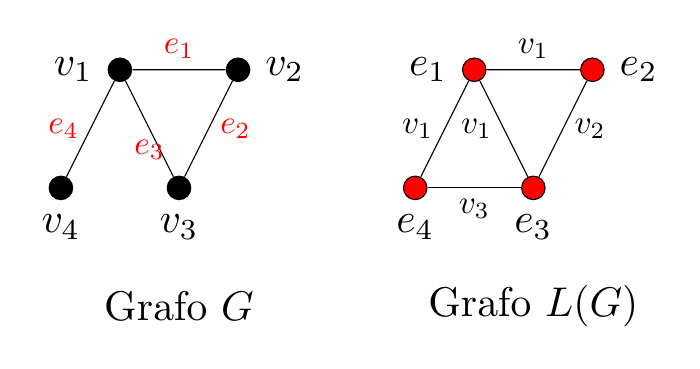
\begin{tikzpicture}[scale=1.5, transform shape]
    % Grafo G
    \node[draw, circle, fill=black, inner sep=2pt, label=left:{$v_1$}] (v1) at (0, 1) {};
    \node[draw, circle, fill=black, inner sep=2pt, label=right:{$v_2$}] (v2) at (1, 1) {};
    \node[draw, circle, fill=black, inner sep=2pt, label=below:{$v_3$}] (v3) at (0.5, 0) {};
    \node[draw, circle, fill=black, inner sep=2pt, label=below:{$v_4$}] (v4) at (-0.5, 0) {};
    \draw (v1) -- node[above, scale=0.8, text=red] {$e_1$} (v2);
    \draw (v2) -- node[right, scale=0.8, text=red] {$e_2$} (v3);
    \draw (v3) -- node[below, scale=0.8, text=red] {$e_3$} (v1);
    \draw (v4) -- node[left, scale=0.8, text=red] {$e_4$} (v1);

    \node at (0.5, -1) {Grafo \(G\)};

    % grafo l(g)
    \node[draw, circle, fill=red, inner sep=2pt, label=left:{$e_1$}] (e1) at (3, 1) {};
    \node[draw, circle, fill=red, inner sep=2pt, label=right:{$e_2$}] (e2) at (4, 1) {};
    \node[draw, circle, fill=red, inner sep=2pt, label=below:{$e_3$}] (e3) at (3.5, 0) {};
    \node[draw, circle, fill=red, inner sep=2pt, label=below:{$e_4$}] (e4) at (2.5, 0) {};
    \draw (e1) -- node[above, scale=0.8, text=black] {$v_1$} (e2);
    \draw (e1) -- node[left, scale=0.8, text=black] {$v_1$} (e3);
    \draw (e1) -- node[left, scale=0.8, text=black] {$v_1$} (e4);
    \draw (e2) -- node[right, scale=0.8, text=black] {$v_2$} (e3);
    \draw (e3) -- node[below, scale=0.8, text=black] {$v_3$} (e4);

    \node at (3.5, -1) {Grafo \(L(G)\)};
\end{tikzpicture}
\end{center}

foi colocado rótulos para facilitar a visualização, mas não é necessários para a definição do grafo.


\hspace*{2em} Como uma carta de uno é um par ordenado de uma cor e um número, as cartas de UNO correspondem ao conjunto de arestas de um grafo bipartido, cujos conjuntos partites são cores e números. Assim, um grafo UNO-1 representa a adjacência de arestas (correspondentes às cartas) de um grafo bipartido. Esses argumentos levam ao seguinte fato.

\begin{tcolorbox}[colback=white, colframe=black!70, title=Lema 1]
se \( g \) é um grafo bipartido, então \( l(g) \) é um grafo de linha.
\end{tcolorbox}

\begin{tcolorbox}[colback=white, colframe=black!70, title=Prova do Lema 1]
\begin{proof}
seja \( g = (v, e) \) um grafo bipartido com partições \( V_1 \) e \( V_2 \). O grafo de linha \( L(G) \) é definido como o grafo cujos vértices são as arestas de \( G \) e duas arestas em \( L(G) \) são adjacentes se e somente se compartilham um vértice em \( G \).

como \( g \) é bipartido, cada aresta \( e \in E \) conecta um vértice de \( V_1 \) a um vértice de \( V_2 \). Portanto, duas arestas \( e_1 \) e \( e_2 \) em \( G \) compartilham um vértice se e somente se uma extremidade de \( e_1 \) está em \( V_1 \) e a outra extremidade está em \( V_2 \), e o mesmo vale para \( e_2 \).

assim, \( l(g) \) é um grafo onde os vértices representam as arestas de \( G \) e duas arestas são adjacentes se compartilham um vértice em \( G \). Portanto, \( L(G) \) é um grafo de linha.
\end{proof}
\end{tcolorbox}

\begin{tcolorbox}[colback=white, colframe=black!70, title=Corolário 1]
\begin{corollary}
se \( g \) é um grafo bipartido, então o problema do Caminho Hamiltoniano em \( L(G) \) é NP-completo.
\end{corollary}
\end{tcolorbox}

\begin{tcolorbox}[colback=white, colframe=black!70, title=Prova do Corolário 1]
\begin{proof}
segue diretamente do teorema 1, que afirma que o problema do Caminho Hamiltoniano para grafos de linha de grafos bipartidos é NP-completo.
\end{proof}
\end{tcolorbox}


\begin{tcolorbox}[colback=white, colframe=black!70, title=Teorema 1]
o problema do caminho hamiltoniano para grafos de linha de grafos bipartidos é NP-completo.
\end{tcolorbox}

portanto, como corolário deste teorema, vemos que UNO é um problema difícil mesmo para um único jogador.

\begin{tcolorbox}[colback=white, colframe=black!70, title=Teorema 2]
uno-1 é np-completo.
\end{tcolorbox}
\textbf{\color{red} melhor essa prova... ponto IMPORTANTE DO TRABALHO}

\textbf{\color{red} {não sei se vale a pena colOCAR AS PROVAS EM ANEXOS}}

para fins de completude, fornecemos uma prova direta e concisa do Teorema 2. Em contraste, a prova em \cite{FSU93} depende adicionalmente de \cite{B81}.

\begin{proof}[demostração]
um grafo cúbico é um grafo no qual todo vértice tem grau 3. Reduzimos do problema do Caminho Hamiltoniano para grafos cúbicos (HP-C), que é conhecido por ser NP-completo \cite{GJT76}.

considere uma instância \( g \) de hp-c. transformamos \( G \) em um grafo \( G' \), onde:
\[ v(g') = \{(x,e) \mid x \in v(g), e = \{x,y\} \in E(G)\} \]
\[ e(g') = \{((x,e),(y,e)) \mid e = \{x,y\} \in E(G)\} \cup \{((x,e_i),(x,e_j)) \mid e_i \neq e_j\} \]

essa transformação divide qualquer vértice \( x \in V(G) \) em três novos vértices \( (x,e_1), (x,e_2), (x,e_3) \) para formar uma clique (triângulo), enquanto cada aresta \( e_i \) (i=1,2,3) incidente a \( x \) torna-se incidente a um novo vértice \( (x,e_i) \). A \autoref{fig:uno1graph} ilustra este "gadget" de nó.


em seguida, preparamos o conjunto de cartas \( C \) do jogador de Uno-1 como o conjunto \( V(G') \), onde a cor e o número de \( (x,e) \) são \( x \) e \( e \), respectivamente. Podemos facilmente confirmar que existe uma aresta \( e = (t,t') \) em \( G' \) se e somente se \( t \) e \( t' \) correspondem. Assim, \( G' \) é o grafo UNO-1 correspondente ao conjunto de cartas \( C \).


agora basta mostrar que existe um caminho hamiltoniano em \( G \) se, e somente se, existe um caminho Hamiltoniano em \( G' \).
\end{proof}


AAAAAAAAAAAAAAAAAAAAAAAAAAAAAAAAAAAAAAAAAAAAAAAAA

O problema do Caminho Hamiltoniano (HP-C) consiste em encontrar um caminho em um grafo que passe por todos os vértices exatamente uma vez. Este problema é bem conhecido por ser NP-completo em diversos tipos de grafos, e será o ponto de partida para a redução que será feita no caso do Uno-1, já que os probelmas são bem semelhante, já que queremos descartar todas as cartas exatamente uma vez.


O objetivo dessa redução é provar que Uno-1 é NP-completo. A ideia principal é reduzir o Problema do Caminho Hamiltoniano para grafos cúbicos (HP-C) para o problema Uno-1, ou seja, mostrar que, dado um grafo cúbico \( G \) (onde cada vértice tem grau 3), podemos transformá-lo em um grafo \( G' \) tal que a existência de um caminho Hamiltoniano em \( G \) é equivalente à existência de um caminho Hamiltoniano em \( G' \). Se conseguirmos isso, então sabemos que o problema de encontrar um caminho Hamiltoniano em Uno-1 é tão difícil quanto o problema do Caminho Hamiltoniano em grafos cúbicos, que é NP-completo, ou seja, depois basta provar que existe dado um conjunto de vétices é possível verificar em tempo polinimial se esses vértices forma um caminho hamiltoniano e demostramos que o problema do Uno-1 é NP-completo.

\textbf{Transformação de \( G \) em \( G' \)(De um grafo cubico para de Uno-1):}

Agora vamos mostrar como é feita a transformação do grafo \( G \) (um grafo cúbico) para o grafo \( G' \) (o grafo correspondente ao jogo Uno-1). A transformação que é feita tem como objetivo alterar a estrutura de \( G \) de modo que cada vértice \( x \) de \( G \) seja substituído por três vértices em \( G' \), formando um clique (ou triângulo). Para faciliar o entendimento queremos fazer o que é mostrado na \autoref{fig:uno1graph}. Vamos ver como isso é feito:

\begin{figure}[hbt]
    \begin{minipage}{1.0\linewidth}
    \centering
    \scalebox{0.75}{\input{grafos/triangle_gadget.tps}}
    \caption{um "gadget" de nó divide um vértice em três vértices para formar um triângulo.}
    \label{fig:uno1graph}
    \end{minipage}
\end{figure}


\begin{itemize}
    \item Para cada vértice \( v \in G \) e para cada aresta \( e = \{v, y\} \in E(G) \), criamos um vértice \( (v, e) \) em \( G' \). Ou seja, cada aresta \( e \) de \( G \) gera um vértice no grafo \( G' \).
    \item As arestas de \( G' \) são formadas de duas maneiras:
    \begin{itemize}
        \item Para cada aresta \( e = \{x, y\} \in E(G) \), adiciona-se uma aresta entre \( (x, e) \) e \( (y, e) \) em \( G' \).
        \item Para cada vértice \( v \in V(G) \), criam-se arestas entre os vértices \( (v, e_1), (v, e_2), (v, e_3) \) para todas as arestas \( e_i \) incidentes a \( v \). Como \( G \) é cúbico, ou seja, cada vértice tem grau 3, então \( v \) será substituído por três vértices em \( G' \), formando um triângulo, com arestas entre \( (v, e_1), (v, e_2), (v, e_3) \).
    \end{itemize}
\end{itemize}

\textbf{Construção do Conjunto de Cartas de Uno-1:}

Depois de criar o grafo \( G' \), é necessário preparar o conjunto de \textit{cartas de Uno-1}, que é composto pelos vértices do grafo \( G' \). Cada carta de Uno-1 tem:
\begin{itemize}
    \item O \textbf{número} da carta que corresponde ao \textbf{x} do vértice \( (x, e) \).
    \item A \textbf{cor} da carta que corresponde á aresta \textbf{e} ou seja, a cor é associada ao vértice original \( x \) de \( G \).
\end{itemize}

Podemos confirmar facilmente que existe uma aresta \( e = (t, t') \) em \( G' \) se, e somente se, \( t \) e \( t' \) combinam, já que só existem duas possibilidades, para a aresta $e$, ou ela está em uma clique ou ela está ligando duas cliques. Caso ela pertença a mesma clique, isso siginica que elas possuem a mesmo número e se elas estão entre clique significa que elas possuema mesma cor. Dois vértices \( t, t' \) em \( G' \) combinam se eles representam cartas que podem ser jogadas consecutivamente no Uno-1, ou seja, compartilham ao menos um atributo (cor ou número). Em expreções matemáticas isso é garantido e expresso pelas seguintes condições:

\begin{itemize}
    \item \( t = (x, e) \) e \( t' = (y, e) \), onde ambos os vértices estão associados à mesma aresta \( e \) de \( G \), ou
    \item \( t = (x, e_i) \) e \( t' = (x, e_j) \), onde \( t \) e \( t' \) pertencem ao triângulo criado para o vértice \( x \) em \( G \).
\end{itemize}

Assim, \( G' \) é o grafo correspondente ao conjunto de cartas \( C \), onde cada vértice \( (v, e) \) em \( G' \) representa uma carta associada ao vértice \( v \) e à aresta \( e \) de \( G \), e as arestas em \( G' \) modelam as combinações válidas de cartas jogáveis.


\textbf{Correlacionando os Caminhos Hamiltonianos:}

Agora, iremos mostrar a relação entre os caminhos Hamiltonianos em \( G \) e \( G' \). Primeiro, suponha que existe um Caminho Hamiltoniano \( P = (v_{i_1}, \dots, v_{i_n}) \) em \( G \). Construímos um Caminho Hamiltoniano \( P' \) em \( G' \) com base em \( P \) da seguinte forma:


\begin{center}
    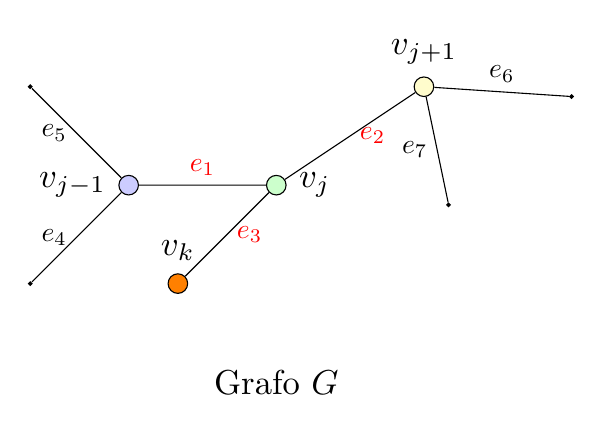
\begin{tikzpicture}[scale=1.25, transform shape]
        % Grafo G
        \node[draw, circle, fill=blue!20, inner sep=2pt, label=left:{$v_{j-1}$}] (v1) at (-0.5, 1) {};
        \node[draw, circle, fill=green!20, inner sep=2pt, label=right:{$v_j$}] (v2) at (1, 1) {};
        \node[draw, circle, fill=yellow!20, inner sep=2pt, label=above:{$v_{j+1}$}] (v3) at (2.5, 2) {};
        \node[draw, circle, fill=black, inner sep=0pt] (v4) at (-1.5, 0) {};
        \node[draw, circle, fill=black, inner sep=0pt] (v5) at (-1.5, 2) {};
        \node[draw, circle, fill=orange, inner sep=2pt, label=above:{$v_k$}] (v6) at (0, 0) {};
        \node[draw, circle, fill=black, inner sep=0pt] (v8) at (4, 1.9) {};
        \node[draw, circle, fill=black, inner sep=0pt] (v9) at (2.75, 0.8) {};
        \draw (v1) -- node[above, scale=0.8, text=red] {$e_1$} (v2);
        \draw (v2) -- node[right, scale=0.8, text=red] {$e_2$} (v3);
        \draw (v2) -- node[right, scale=0.8, text=red] {$e_3$} (v6);
        \draw (v4) -- node[left, scale=0.8] {$e_4$} (v1);
        \draw (v5) -- node[left, scale=0.8] {$e_5$} (v1);
        \draw (v3) -- node[above, scale=0.8] {$e_6$} (v8);
        \draw (v3) -- node[left, scale=0.8] {$e_7$} (v9);
    
        \node at (1, -1) {Grafo \(G\)};
    \end{tikzpicture}
    \end{center}
    
    \begin{center}
        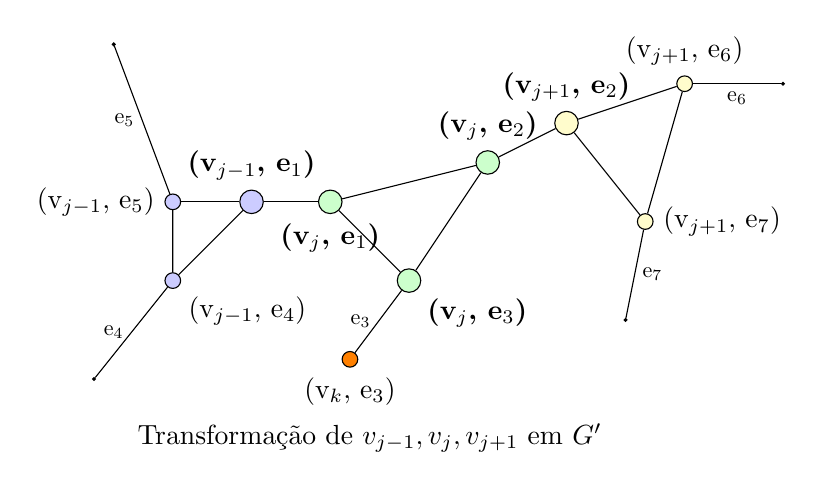
\begin{tikzpicture}[scale=1, transform shape]
            % Transformação em G'
            % v_{j-1}
            \node[draw, circle, fill=blue!20, inner sep=2pt, label=left:{(v\(_{j-1}\), e\(_5\))}] (v1_e1) at (-1.5, -0.5) {};
            \node[draw, circle, fill=blue!20, inner sep=2pt, label=below right:{(v\(_{j-1}\), e\(_4\))}] (v1_e2) at (-1.5, -1.5) {};
            \node[draw, circle, fill=blue!20, inner sep=3pt, label=above:{\textbf{(v\(_{j-1}\), e\(_1\))}}] (v1_e3) at (-0.5, -0.5) {};
            \node[draw, circle, fill=black, inner sep=0pt] (e1) at (-2.25, 1.5) {};
            \node[draw, circle, fill=black, inner sep=0pt] (e2) at (-2.5, -2.75) {};
            \draw (v1_e1) -- (v1_e2) -- (v1_e3) -- cycle; % Triângulo de v_{j-1}
            \draw (v1_e1) -- (v1_e3); % Aresta adicional no triângulo
        
            % v_j
            \node[draw, circle, fill=green!20, inner sep=3pt, label=below:{\textbf{(v\(_j\), e\(_1\))}}] (v2_e3) at (0.5, -0.5) {};
            \node[draw, circle, fill=green!20, inner sep=3pt, label=below right:{\textbf{(v\(_j\), e\(_3\))}}] (v2_e4) at (1.5, -1.5) {};
            \node[draw, circle, fill=green!20, inner sep=3pt, label=above:{\textbf{(v\(_j\), e\(_2\))}}] (v2_e6) at (2.5, 0) {};
            \node[draw, circle, fill=orange, inner sep=2pt, label=below:{(v\(_k\), e\(_3\))}] (e4) at (0.75, -2.5) {};
            \draw (v2_e3) -- (v2_e4) -- (v2_e6) -- cycle; % Triângulo de v_j
            \draw (v2_e3) -- (v2_e6); % Aresta adicional no triângulo
        
            % v_{j+1}
            \node[draw, circle, fill=yellow!20, inner sep=3pt, label=above:{\textbf{(v\(_{j+1}\), e\(_2\))}}] (v3_e6) at (3.5, 0.5) {};
            \node[draw, circle, fill=yellow!20, inner sep=2pt, label=right:{(v\(_{j+1}\), e\(_7\))}] (v3_e7) at (4.5, -0.75) {};
            \node[draw, circle, fill=yellow!20, inner sep=2pt, label=above:{(v\(_{j+1}\), e\(_6\))}] (v3_e8) at (5.0, 1) {};
            \node[draw, circle, fill=black, inner sep=0pt] (e7) at (4.25, -2) {};
            \node[draw, circle, fill=black, inner sep=0pt] (e8) at (6.25, 1) {};
            \draw (v3_e6) -- (v3_e7) -- (v3_e8) -- cycle; % Triângulo de v_{j+1}
            \draw (v3_e6) -- (v3_e8); % Aresta adicional no triângulo

            % % v_k
            % \node[draw, circle, fill=orange, inner sep=3pt, label=above:{\textbf{(v\(_k\), e\(_3\))}}] (vk_e3) at (0.75, 1) {};
            % \draw (vk_e3) -- (v2_e3); % Aresta adicional no triângulo


        
            % Conexões entre vértices (v, e) e (y, e) (arestas compartilhadas)
            \draw (v1_e3) -- (v2_e3); % Aresta compartilhada entre v_{j-1} e v_j
            \draw (v2_e6) -- (v3_e6); % Aresta compartilhada entre v_j e v_{j+1}
        
            % Conexões específicas para as novas arestas
            \draw (e2) -- node[left, scale=0.8] {e\(_4\)} (v1_e2);
            \draw (e1) -- node[left, scale=0.8] {e\(_5\)} (v1_e1);
            \draw (e4) -- node[left, scale=0.8] {e\(_3\)} (v2_e4);
            \draw (e7) -- node[right, scale=0.8] {e\(_7\)} (v3_e7);
            \draw (e8) -- node[below, scale=0.8] {e\(_6\)} (v3_e8);
        
            % Label
            \node at (1, -3.5) {Transformação de \(v_{j-1}, v_j, v_{j+1}\) em \(G'\)};
        \end{tikzpicture}
    \end{center}
    



Pode-se verificar que o caminho \( P' \) em \( G' \) assim formado é Hamiltoniano.

Agora, para o caso inverso, suponha que existe um Caminho Hamiltoniano \( P' \) no grafo \( G' \). Se \( P' \) visita os vértices \( (v, e_i) \) (\( i = 1, 2, 3 \)) consecutivamente em qualquer ordem, como mostrado em \autoref{fig:possible_tours} (a1) ou (a2), então \( P' \) pode ser diretamente transformado em um Caminho Hamiltoniano \( P \) em \( G \), bastando mapear \( (v, e_i) \) para \( v \).

Se \( P' \) não visitar \( (v, e_i) \) consecutivamente, existem dois casos, como ilustrado em \autoref{fig:possible_tours} (b') e (c'). Nesses casos, pelo menos uma extremidade de \( P' \) é da forma \( (v, e_i) \). Podemos reorganizar \( P' \) para garantir que os vértices \( (v, e_i), (v, e_j), (v, e_k) \) sejam visitados consecutivamente, como mostrado em \autoref{fig:possible_tours} (b) e (c), sem afetar a Hamiltonicidade do caminho.

Assim, demonstramos que \( P' \) pode ser transformado em um Caminho Hamiltoniano em \( G \), concluindo a equivalência entre os dois problemas.
    


\begin{figure}[hbt]
    \begin{minipage}{1.0\linewidth}
    \centering
    \scalebox{0.75}{\input{grafos/possible_tours.tps}}
    \caption{Possibilidade de caminhos passando por cada nó "gadget".}
    \label{fig:possible_tours}
    \end{minipage}
\end{figure}

Com esses argumentos, mostramos que a existência de um caminho Hamiltoniano em \( G \) é equivalente à existência de um caminho Hamiltoniano em \( G' \). Como o problema do Caminho Hamiltoniano em grafos cúbicos é NP-completo, isso implica que o problema Uno-1 também é NP-completo. Portanto, Uno-1 é NP-completo.
